

\section{Maps}
Maps were designed in a top-down view. The only limitation was that walls were perpendicular to floors. Everything was done in 2D. A designed worked with just five types of elements: \cw{VERTEX}\footnote{Vertices coordinates were expressed with signed short integer [-32768, 32767]}, \cw{LINE}, \cw{SIDEDEF}, \cw{SECTOR}, and \cw{THING}.\\
\par
\drawing{doom_map_basics}{}

\par
A \cw{SECTOR} is a closed area surrounded by \cw{LINE}s with a specified floor height, floor texture, ceiling height, ceiling texture, and a light level. A sector can be concave, but lines cannot cross each others.\\
\par
A \cw{LINE} can either be a solid wall or a portal between two \cw{SECTOR}s. The difference is in the number of \cw{SIDEDEF} associated with it. A wall has only one \cw{SIDEDEF} on its right side and is fully opaque. A portal has two \cw{SIDEDEF}s and can usually be partially seen though.\\
\par
A \cw{SIDEDEF} describes one side of a line. To accommodate walls and portals texturing it can have up to three textures. The middle texture is used by wall for the full area they cover. There can also have lower texture and an upper texture for portal connecting \cw{SECTOR}s with different ceiling/floor height. If the portal leads to a sector with higher floor, the lower texture is used to render the "step". If the \cw{SECTOR} connects to a \cw{SECTOR} with lower ceiling, the upper texture is used to render the "down step". To help alignment with door and buttons, \cw{SIDEDEF} textures can have a vertically/horizontally offset. \\
\par
A \cw{THING} is must simpler in comparison. It only has one \cw{VERTEX} coordinate, an angle and an identifier telling its type. As the minimum a map must have one player spawning location \cw{THING}.\\

\cfullimage{doom_map.png}{Rendering of map shown in figure \ref{doom_map_basics}.}
\par
The resulting scene in figure \ref{doom_map.png} is ugly but the mismatched colors hopefully help to dissociate each elements. All \cw{LINE}s are walls except for \cw{E-B} which has two \cw{SIDEDEF}s and is therefore a portal. All walls use the \cw{BRIK} middle texture except for the portal which uses \cw{GRAY} for both top and bottom.\\
\par
\cw{SECTOR} \#0 uses a \cw{RED} floor texture and a \cw{WOOD} ceiling texture. The height of the floor is 20 and its ceiling is at 40. \cw{SECTOR} \#1 uses a \cw{BLUE} floor texture and a \cw{GREN} ceiling texture. Its floor is at 60 and ceiling at 60. Both sectors have the same light level (10).\\
\par
   Notice the portal \cw{E-B} which does not have a mid-texture but an upper and lower texture. These were used to draw the up-step and down-step towards sector \#0.\\
\par
Also notice the wall \cw{D-E} which mid-texture vertical offset was not correctly set, resulting in a vertical tear when connecting with wall \cw{E-F}. Wall \cw{B-C} vertical offset was properly set and result in no visual artifact. None of the wall use an horizontal offset, however field is marked \cw{XOFF} on figure \ref{doom_map_basics} to show its location.\\ 
\pagebreak



\subsection{Map Editor (DoomED)}
To harness the complexity of the map format, a new tool was created. The Doom map EDitor was to be called \textbf{DoomED}. This is were \NeXT solution asserted the most impact. The high resolution of the display allowed a lot of real-estate showing small details and many widgets. The stability of NeXTSTEP allowed to never lose work while writing DoomED or creating a map.
The very design of Objective-C also had a tremendous influence. The language's message dispatching system no-op behavior when dereferencing a \cw{nullptr}\footnote{"Understanding the Objective-C Runtime".} created a fault forgiving environment where a faulty feature would not work but did not crash either.\\
\par   
The killing feature was Application Builder which not only came with a full library of widgets but also allowed to create new one and connect them to the business logic instantly.\\
\par
\fullimage{doomed/DoomEd.png}
\par

The release of the source code in April 2015 allowed to pick inside. There is almost as much code as in the game engine (doom:32kloc, DoomED:20kcloc). Without the power of \NeXT the editor would have taken at least twice the same amount of time to make.



\tcode{cloc_doomed.txt}
\par
DoomED was designed to be the "Adobe Illustrator for World Maps" where the designer simply drew line, selected sectors , and picked textures. A skilled map maker could complete a map in 20 minutes \fixme{citation needed JOHN?}.\\
\par

\trivia{DoomED icon is an Imp. Upon startup a growling sound is played.}\\
\par
\fullimage{doomed/all_widgets.png}


\vspace{-4mm}
DoomED did not output data usable by the game engine directly. Instead it generated a text format output called \cw{DWD}. A header served as magic number which was followed by a list of lines listing sidedefs and a list of things. Sectors were inferred from line's ceiling/floor textures values.\\
\par
\tcode{map.txt}
\par
DWD was not designed with space efficiency in mind but rather to be easy to parse since it was processed by a Node Builder tool \cw{doombsp}.\\
\par
\cfullimage{props/tom.png}{Tom Halls, delighted next to his NeXTCube running DoomED. The sticker on the monitor spells "quality".}
\par

\pagebreak





\section{Map Preprocessor (Node Builder)}
Map preprocessing was not something new at id. In 1991 with Wolfenstein 3D maps were already pre-processed to allow fast sound propagation. With \doom, it was taken to a whole new level both in terms of complexity and processing time.\\
\par
The main issue at hand was to maintain the same rendering speed despite relaxing the orthogonal grid constraint of Wolfenstein and losing usage of the DDA algorithm \footnote{Digital Differential Analyzer was used extensively for VSD (Visual Surface Determination), collision detection and light of sight calculation. This was all gone with \doom.}. The solution chosen was to create for each map a multitude of accelerating data structures, each dedicated to solving a particular problem.\\
\par
 The tool to do that was called \cw{doombsp}. It took as input a \cw{.DWD} map and outputted a \cw{.WAD}. Not only the map was expressed in a space efficient manner (e.g: Expressing vertices only once and referencing them via index), three sections were generated alongside. A Binary Space Partitioned version of the map expressed a node tree to speed up rendering. A blockmap meant to accelerate collision detection. And finally a reject table to accelerate A.I processing.\\
 \par
\trivia{Map preprocessing took a significant amount of time. With a NextStation Turbo Color, running \cw{doombsp} on \cw{E1M1} took 10s. On E1M2, it took 30s. On E2M7, it took a full minute. The first nine maps of the shareware took 3mn26s. The full twenty seven maps of the registered version took 11mn.}\\% This was a problem for designers...yet it was little compared to what Quake's \cw{qbsp} would be three years later.}\\
\par
\tcode{cloc_doombsp.txt}
\par
 \trivia{\cw{DoomED.app}, \cw{doom} and \cw{doombsp} were tightly integrated. One button in the editor was enough to save the map, invoke the nodebuilder and start the game with the WIP map.}


%
\begin{figure}[H]
\vspace*{3mm}
\centering
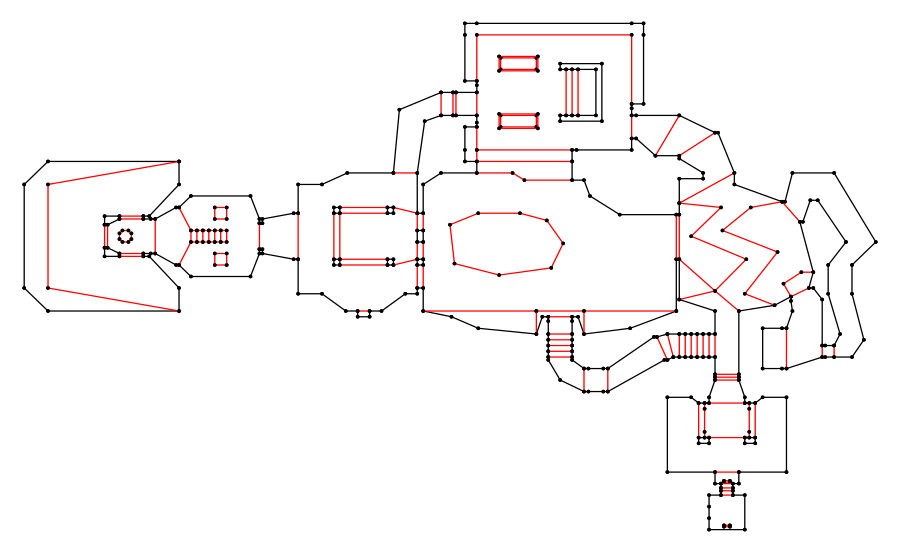
\includegraphics[width=\textwidth]{drawings/E1M1_lines.pdf}
\end{figure}
\par
The map as it is generated via DoomED.\\
\par
\begin{figure}[H]
\vspace*{2mm}
\centering
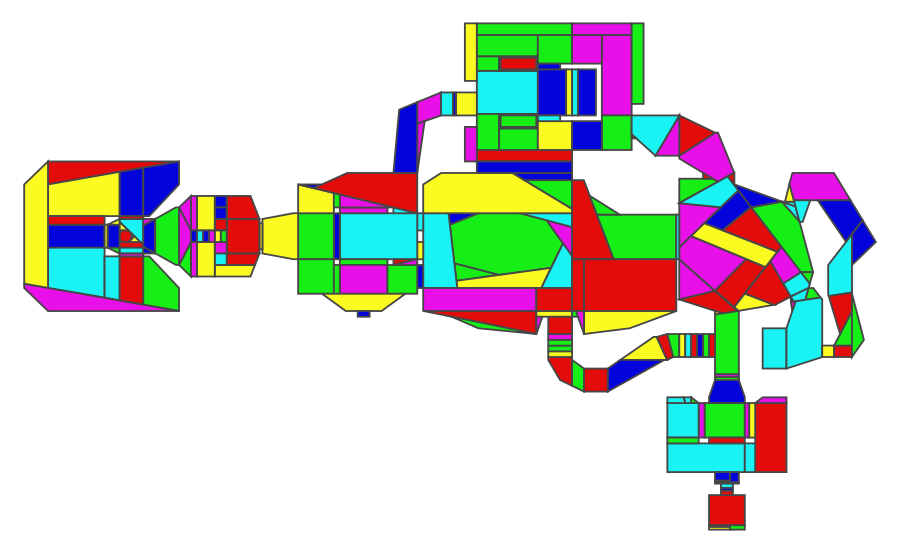
\includegraphics[width=\textwidth]{drawings/E1M1_fab.pdf}
\end{figure}
The BSP node tree where all sectors become convex sub-spaces called sub-sectors.



\begin{figure}[H]
\centering
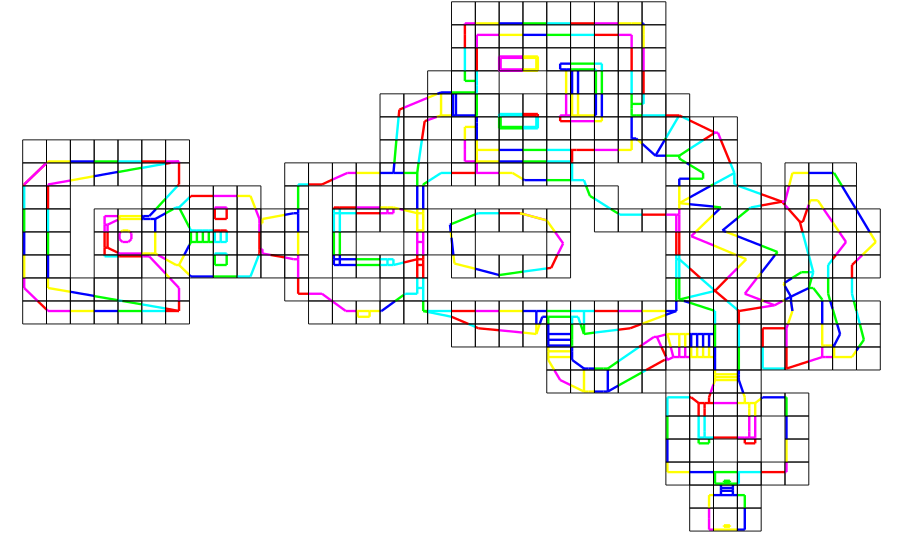
\includegraphics[width=\textwidth]{drawings/E1M1_blockmap.pdf}
\end{figure}
\par
Blockmap slicing where each block is 128x128 to accelerate collision detections.\\
\par
\begin{figure}[H]
\centering
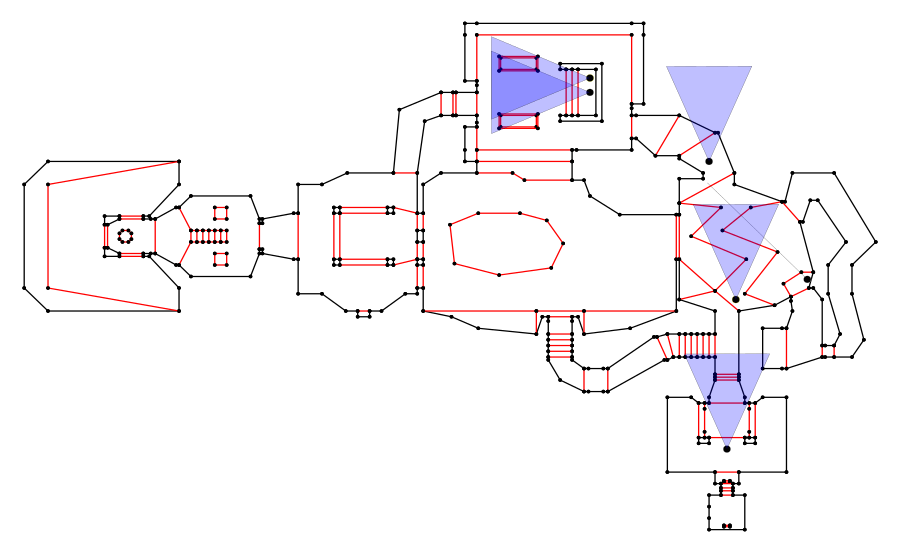
\includegraphics[width=\textwidth]{drawings/E1M1_sides.pdf}
\end{figure}
\par
The Reject datastructure based on enemies and monsters line of sight.
\pagebreak


The source code of the node builder was released shortly after the game in May 1994. It was the NeXTSTEP version but it was quickly converted to DOS and released under the name IDBSP to the delight of a hoard of modders.\\
\par
\cfullimage{doombsp_compiling.png}{Building doombsp on NeXTSTEP.}
\par
For each \cw{.dwd}, \cw{doombsp} outputs a set of lumps and store them in a \cw{.wad} file (see p\pageref{wad_explained}).\\

\par
 \begin{figure}[H]
\centering  
\begin{tabularx}{\textwidth}{ L{0.15} L{0.75} }
  \toprule
  \textbf{Lump Name} &  \textbf{Explanation} \\
  \toprule 
   
   \cw{EXMY} & Map start marker where X is the episode and Y the map number. All subsequent lumps are part of this map "block".\\
   \cw{MAPXY} & Same as EXMY but used in Doom II.\\
   \cw{VERTEXES} & An array of \cw{signed short} X, Y pairs. All coordinates in this map block are indexes into this array.\\
   \cw{LINEDEFS} & An array of lines referencing two vertices. This is a direct translation of the lines used in DoomED. Also points to one or two \cw{SIDEDEFS} depending if this line is a wall or a portal. \\
   \cw{SIDEDEFS} & Defines upper, lower, and middle texture. Also define texture horizontal and vertical offsets.\\
   \cw{SECTORS} & Area surrounded by lines, with set ceiling and floor textures/heights with light level.\\
   \cw{THINGS} & Position and angle for a each monsters, powerup and spawn locations.\\
   \toprule
   \cw{NODES} & BSP with segs nodes and sub-sector leaves.\\
   \cw{SEGS} & Portion of lines cut due to Binary Space Partitioning (see page \pageref{Binary Space Partitioning: Theory}).\\
   \cw{SSECTORS} & Set of \cw{SEGS} representing a convex subspace.\\
   \toprule
   \cw{REJECT} & Sector to sector matrix of what monsters can potentially see in their spawing positon.\\
   \toprule
   \cw{BLOCKMAP} & 128x128 AABB partition of the map \cw{LINEDEFS} to accelerate collision detections.\\
   \toprule
\end{tabularx}
%\caption{Map Data lumps]\protect\footnotemark.}
\end{figure}
\par
\footnotetext{Source:The Unofficial Doom Specs v1.666.}

Slicing the map via binary partitioning is non-trivial. \cw{doombsp} heuristic attempts to minimize the number of segments generated while generating a balanced tree and picking axis aligned splitting lines. A debug flag \cw{-draw} allowed to monitor what was happening. BSP trees and Binary partitioning are explained in details on page \pageref{Binary Space Partitioning: Theory}. \\
\par
\cfullimage{doombsp_run.png}{Running doombsp in debug mode show splitter selection.}
\par
